% LaTeX manuscript for npj Microgravity
% Study-aware re-analysis of Arabidopsis spaceflight transcriptomes with CFD of the flight hardware
% Rewritten 2026-10 to match reports/HEADLINE_2026-10.md; every number traces to
% tables/reanalysis_2026-10/REANALYSIS.md or LunarLeaf-CFD tables named in the text.
\documentclass[11pt,a4paper]{article}

% Packages
\usepackage[utf8]{inputenc}
\usepackage[T1]{fontenc}
\usepackage{lmodern}
\usepackage[margin=2.5cm]{geometry}
\usepackage{graphicx}
\usepackage{booktabs}
\usepackage{tabularx}
\usepackage{multirow}
\usepackage{amsmath,amssymb}
\usepackage{hyperref}
\usepackage{xcolor}
\usepackage{caption}
\usepackage{subcaption}
\usepackage{natbib}
\usepackage{setspace}
\usepackage{lineno}
\usepackage{rotating}
\usepackage{array}

% Hyperref settings
\hypersetup{
    colorlinks=true,
    linkcolor=blue,
    citecolor=blue,
    urlcolor=blue
}

% Line numbering for submission
\linenumbers

% Title
\title{Spaceflight transcriptome responses in \textit{Arabidopsis thaliana} are largely study-specific: a study-aware re-analysis of NASA OSDR data with fluid dynamics of the flight growth hardware}

% Authors
\author{
Richard Barker$^{1,2}$ \\
$^{1}$LunarLeaf-CFD, Open Science Project \\
$^{2}$virtual-root Systems Biology Project \\
\texttt{ORCID: TODO}
}

\date{}

\begin{document}

\maketitle

% ============================================================
\begin{abstract}
Spaceflight transcriptome studies of \textit{Arabidopsis} differ in hardware, tissue, platform and flight, and their results rarely agree. We re-analysed 307 samples from 11 NASA Open Science Data Repository (OSDR) studies with study-aware models, and coupled them to lattice-Boltzmann computational fluid dynamics (CFD) of the BRIC, CARA and VEGGIE growth hardware. A flight response shared by all studies explained under 1\% of gene variance (0.3\% pooled, 0.6\% in RNA-seq alone), against 8--12\% for study-specific flight effects. Within BRIC, flight signatures agreed between the RNA-seq studies (median $r = 0.40$) but not with the earlier microarray studies, which detected almost no flight response. CFD-predicted boundary-layer conductance and carbon supply were confounded with study and did not explain which studies responded: no pathway showed a flight effect or a CFD dose-response in study-aware models. Consistent with this, the CFD shows that inside the flight dishes gravity changes leaf gas exchange only 1.25--1.8-fold, against 2.25-fold in open air, and that sealed BRIC dishes become carbon-limited on the ground as well as in orbit. Spaceflight responses are real but largely experiment-specific, which argues for replicated flights in common hardware rather than pooled meta-analysis.
\end{abstract}

\textbf{Keywords:} spaceflight, \textit{Arabidopsis}, transcriptomics, meta-analysis, study heterogeneity, computational fluid dynamics, boundary layer, NASA OSDR

% ============================================================
\section*{Introduction}

Spaceflight alters gene expression in \textit{Arabidopsis}, and the NASA OSDR now holds transcriptomes from many flight experiments \citep{paul2017}. These experiments used different growth hardware: sealed Petri-dish canisters (BRIC), semi-permeable dishes (CARA) and vented chambers with forced airflow (VEGGIE). They also differ in tissue, ecotype, lighting, plant age and measurement platform. Pooling them promises statistical power, but only if a common flight response exists to be found.

Growth hardware also sets the atmosphere around the plant. In microgravity buoyant convection is lost, so air movement around a leaf depends on ventilation, and forced airflow can restore gas exchange \citep{kitaya2003,monje2005}. If hardware-dependent gas exchange shaped the flight response, quantities predicted by CFD of each hardware, such as the leaf boundary-layer conductance $g_{bl}$, should explain which experiments respond and how strongly.

We asked three questions. (1) How much of the transcriptional variation in pooled spaceflight data is a flight response shared by all studies? (2) Do flight signatures replicate between studies, and does measurement platform matter? (3) Do CFD-predicted gas-exchange quantities explain differences between studies once study structure is respected?

% ============================================================
\section*{Results}

\subsection*{Data and harmonisation}

We analysed 307 expression samples (153 flight, 154 ground control) from 11 OSDR studies: 213 RNA-seq samples from 7 studies and 94 microarray samples from 4 studies (Fig.~\ref{fig:design}). Studies were grouped into three CFD hardware classes: BRIC, CARA and VEGGIE. Two other systems were folded into these classes: APEX-TAGES (OSD-7) into BRIC, and EMCS (OSD-314) into VEGGIE. CARA is represented by a single study (OSD-120).

We rebuilt the harmonised expression matrix from the 11 OSDR processed files and reproduced the original limma-voom fit: 25,453 genes, inter-study correlation 0.7327 against 0.7324, and $t$-statistic correlation 0.999. The original pipeline joined the platforms on gene identifiers and set genes not measured in a study to zero. We therefore repeated the main analyses without zero-filling, and with RNA-seq and microarray modelled separately (Methods).

\subsection*{The flight response is largely study-specific}

We partitioned each gene's variance with every factor as a random effect and hardware nested in study (Fig.~\ref{fig:vp}).
\begin{itemize}
    \item \textbf{Study} explained 53.3\% of the average gene's variance in the pooled data (17,129 genes measured in all studies) and 44.8\% in the RNA-seq studies alone (23,531 genes).
    \item \textbf{A flight effect common to all studies} explained 0.3\% and 0.6\%.
    \item \textbf{Study-specific flight effects} explained 8.3\% and 11.9\%.
\end{itemize}
Only 10 of 17,129 genes (71 of 23,531 in RNA-seq) had more than 10\% of their variance in the common flight effect, against 4,597 and 8,899 in flight $\times$ study. Spaceflight changes expression substantially within experiments, but mostly in ways that differ between them.

\subsection*{Pooled flight contrasts depend on the reference hardware}

In a factorial limma-voom model ($\sim$ flight $\times$ hardware + organ + light + ecotype, with study as a correlated block), the default flight coefficient is the flight effect in the reference hardware, BRIC: 11,675 genes at FDR $< 0.05$. The flight effect averaged over BRIC, CARA and VEGGIE involved 4,598 genes (285 with $|\log_2\mathrm{FC}| > 1$), and the two estimates agreed only weakly across genes ($r = 0.35$). Restricting to genes measured in every study changed these counts little (10,831 and 3,637). Which hardware is taken as the reference therefore largely determines what a pooled ``flight effect'' contains.

\subsection*{Flight signatures replicate between BRIC RNA-seq studies, not with microarray studies}

Within BRIC, the RNA-seq and microarray flight effects were uncorrelated ($r = -0.05$). Platform is confounded with study and organ, so we estimated the flight effect separately in each study $\times$ organ unit and compared units from different studies (Fig.~\ref{fig:platform}).
\begin{itemize}
    \item The three BRIC RNA-seq studies agreed with one another (median $r = 0.40$).
    \item The BRIC microarray studies agreed neither with each other (median $r = 0.01$) nor with the RNA-seq studies ($-0.03$; whole seedlings only, $-0.04$).
    \item The microarray units detected a median of 5.5 flight genes at FDR $< 0.05$, against 7,381 in the BRIC RNA-seq units.
\end{itemize}
The platform split is therefore weak or absent flight signal in the microarray studies, not an opposite response. These are the earlier BRIC flights, so platform and flight era cannot be separated. Across hardware, even RNA-seq studies agreed poorly (median $r = 0.09$).

\subsection*{CFD covariates do not explain which studies respond}

Each CFD covariate takes one value per hardware $\times$ gravity $\times$ organ-scale cell, so neither can be separated from study.
\begin{itemize}
    \item \textbf{$g_{bl}$} relabels the flight $\times$ organ-scale cells (variance inflation factor 13.6).
    \item \textbf{Carbon supply} is a hardware label once BRIC ground controls are given the sealed-dish value: study membership explains 99.9\% of its variance.
\end{itemize}

At the pathway level, we scored 28 curated pathways within each study on each platform's own log scale. These scores avoid zero-filling and count each gene once. We then fitted a within-study model with cluster-robust standard errors by study.
\begin{itemize}
    \item \textbf{Flight:} no pathway showed a flight effect at FDR $< 0.05$ (Fig.~\ref{fig:pathways}).
    \item \textbf{Organ scale:} three pathways differed between rosette and leaf scale: ethylene biosynthesis, jasmonate signalling and gravitropism signalling.
    \item \textbf{CFD dose-response:} a meta-regression of study-level flight effects on the CFD-predicted boundary-layer penalty (14 study $\times$ scale units, Knapp--Hartung inference) found no pathway at FDR $< 0.05$.
    \item \textbf{Power:} a planted flight effect of 0.25 or 0.5 within-study SD was detected in 8/28 and 15/28 pathways, so these tests rule out only large effects.
\end{itemize}

\subsection*{Inside the flight dish, gravity matters less than open-air models suggest}

LunarLeaf-CFD resolves the leaf boundary layer at 0.288~mm in two dimensions, with buoyancy driven by CO\textsubscript{2}, O\textsubscript{2} and H\textsubscript{2}O concentration differences (Fig.~\ref{fig:cfd}).
\begin{itemize}
    \item \textbf{Open box:} a leaf's $g_{bl}$ falls from 0.997 at 1\,g to 0.443\,mol\,m\textsuperscript{-2}\,s\textsuperscript{-1} at 0\,g, a 2.25-fold penalty (LunarLeaf-CFD T13).
    \item \textbf{Real dishes:} inside the BRIC 60\,mm and CARA 120\,mm dishes, the shallow headspace keeps convection weak even at 1\,g, and the penalty shrinks to 1.25--1.8-fold (T19).
    \item \textbf{At 0\,g:} both dishes give nearly the same conductance to their own air (0.185 and 0.186).
    \item \textbf{Sealed BRIC dish:} with photosynthesis feedback, it runs out of CO\textsubscript{2} in about 3.5\,min at either gravity (T20). With humidity-limited transpiration, its 1\,g and 0\,g boundary layers converge within minutes (T22).
\end{itemize}
In the sealed hardware, ground controls are therefore carbon-limited too, and the gravity contrast in gas exchange is small. That is consistent with the absence of a boundary-layer dose-response in the transcriptomes.

\subsection*{Exploratory analyses}

The original pipeline also deconvolved the bulk samples against the Shahan root atlas (GSE152766) \citep{shahan2022} with a scVI model \citep{lopez2018}, and inferred miRNA activity from target-gene expression. Both were run on the zero-filled matrix; the deconvolution uses a root-only reference for mostly non-root samples. The miRNA analysis covered 19 miRNAs across 34 contrasts, and no target set was enriched among differentially expressed genes (all FDR $= 1$). We report these analyses in the supplementary tables but do not interpret them.

% ============================================================
\section*{Discussion}

The pooled OSDR data contain a large flight response within experiments but very little that is shared between them. A flight effect common to all studies explains under 1\% of gene variance, against 8--12\% for study-specific flight effects. Pooled contrasts are therefore fragile: the default ``flight effect'' of a factorial model is the effect in the reference hardware, and an estimate averaged over hardware differs substantially. Within one hardware, the RNA-seq studies do share a flight signature. This suggests that common biology exists, but is masked by differences in hardware, tissue, platform and flight.

The microarray studies contribute almost no flight signal. Whether this reflects the platform or the earlier flights cannot be decided with these data, but it means that pooling the two platforms dilutes rather than strengthens a flight signature.

The CFD covariates did not explain which studies respond. With so few independent studies per hardware, any hardware-level covariate is confounded with study by construction. The CFD itself also predicts a small effect: inside the flight dishes, the gravity penalty on leaf gas exchange is modest. In sealed BRIC dishes, carbon limitation is a property of the hardware, shared by flight and ground. Hardware atmospheres may well shape plant responses, but testing that needs replicated flights in common hardware, with ground controls in identical enclosures, rather than covariates applied after the fact to heterogeneous experiments.

\textbf{Limitations.}
\begin{itemize}
    \item Hardware is nested in study, and CARA is a single study.
    \item APEX-TAGES and EMCS were folded into the BRIC and VEGGIE classes.
    \item The positive controls show that the pathway tests can rule out only large effects.
    \item The CFD is two-dimensional, its humidity saturation level is an estimate, and it is not yet validated against in-flight measurements.
\end{itemize}

% ============================================================
\section*{Methods}

\subsection*{Data}

Processed expression files for 11 OSDR studies were downloaded from the OSDR biodata API. For the 7 RNA-seq studies these were the GeneLab normalised counts and RSEM expected counts; for the 4 microarray studies, the normalised probe-set intensities. A manifest with source URLs and SHA-256 checksums accompanies the code. Sample metadata (ecotype, organ, flight, light, hardware) follows the original OSDR harmonisation; organ was mapped to leaf or rosette CFD scale.

\subsection*{Harmonisation}

Microarray probe sets were mapped to AGI identifiers and averaged per gene. The original matrix was an outer join of all studies with unmeasured genes set to zero, and was rebuilt to reproduce the stored fit. Two corrected variants were analysed:
\begin{itemize}
    \item \textbf{complete case:} genes measured in every study (17,129);
    \item \textbf{platform-separated:} RNA-seq modelled with voom on RSEM expected counts (TMM normalisation \citep{robinson2010}, low-count filtering), and microarray with limma-trend on the published log\textsubscript{2} intensities.
\end{itemize}

\subsection*{Differential expression}

Models were fitted with limma-voom \citep{law2014,smyth2005}, with study as a correlated block estimated by duplicateCorrelation \citep{smyth2005b}.
\begin{itemize}
    \item \textbf{Factorial model:} $\sim$ flight $\times$ hardware + organ + light + ecotype. The flight effect averaged over hardware was tested as a contrast giving each hardware equal weight.
    \item \textbf{CFD-covariate model:} replaced hardware with $g_{bl}$ and carbon supply. Collinearity was assessed with variance inflation factors and with the variance of each covariate explained by study.
\end{itemize}
False discovery rates used the Benjamini--Hochberg procedure \citep{benjamini1995}.

\subsection*{Variance partitioning}

Variance components were estimated per gene with variancePartition \citep{hoffman2016}, using the formula $\sim$ (1$|$hardware) + (1$|$study) + (1$|$flight) + (1$|$flight:hardware) + (1$|$flight:study) + (1$|$organ) + (1$|$light) + (1$|$ecotype). It was applied to voom-weighted complete-case data and to the RNA-seq studies alone. The CFD covariates were omitted, because their canonical correlation with study is 1.00.

\subsection*{Platform concordance}

The flight effect was estimated separately in each study $\times$ organ unit with at least two flight and two ground samples. The model was flight plus ecotype and light where these varied within the unit (voom for RNA-seq, limma-trend for microarray). Concordance was the Pearson correlation of $\log_2$ fold changes over shared genes, summarised for pairs of units from different studies.

\subsection*{Pathway scores and models}

The 28 curated gene sets were checked against UniProt. Repeated entries were removed, one misassigned gene was removed from the heat-shock set, and the heat-shock transcription factors and HSP101 were added. Scores were computed within each study as the mean within-study $z$-score of member genes. RNA-seq expression was taken as log\textsubscript{2} counts per million, and microarray as published log\textsubscript{2} intensities.

Each pathway score was modelled as $\sim$ study + flight $\times$ scale, with effect coding. Standard errors were cluster-robust (CR1) by study \citep{cameron2015}, with $t$ tests on $G - 1$ degrees of freedom; terms identified within fewer than two studies were not tested. Study-level flight effects were meta-regressed on the CFD-predicted penalty with Knapp--Hartung inference \citep{knapp2003}. Positive controls added a known flight effect to every pathway and recorded detection.

\subsection*{CFD}

Boundary-layer quantities come from LunarLeaf-CFD, a two-dimensional D2Q9 lattice-Boltzmann solver with D2Q5 transport of CO\textsubscript{2}, O\textsubscript{2} and H\textsubscript{2}O and concentration-driven buoyancy. Leaf and rosette scenes were run to steady state (T13). The real BRIC and CARA dish cross-sections were modelled with the leaf 1\,mm above the agar (T19). Sealed-dish runs added CO\textsubscript{2}-limited photosynthesis (T20) and humidity-limited transpiration (T22). Covariates were assigned per sample by hardware class, gravity (flight = 0\,g) and organ scale.

\subsection*{Code and data availability}

All code, tables and figures are at \url{https://github.com/dr-richard-barker/Airflow_omics}. The CFD model is at \url{https://github.com/dr-richard-barker/LunarLeaf-CFD}. Expression data are from NASA OSDR (\url{https://osdr.nasa.gov}). The full analysis record, with every number in this manuscript, is \texttt{tables/reanalysis\_2026-10/REANALYSIS.md}. Archival DOI: TODO.

% ============================================================
\section*{Acknowledgments}

We thank the NASA GeneLab and OSDR teams for maintaining open-access spaceflight omics data, and the \textit{Arabidopsis} single-cell genomics community for making reference atlases publicly available.

% ============================================================
\section*{Author contributions}

R.B. conceived the study, developed the CFD model, performed all analyses, and wrote the manuscript.

% ============================================================
\section*{Competing interests}

The author declares no competing interests.

% ============================================================
% Figures
% ============================================================

\begin{figure}[htbp]
\centering
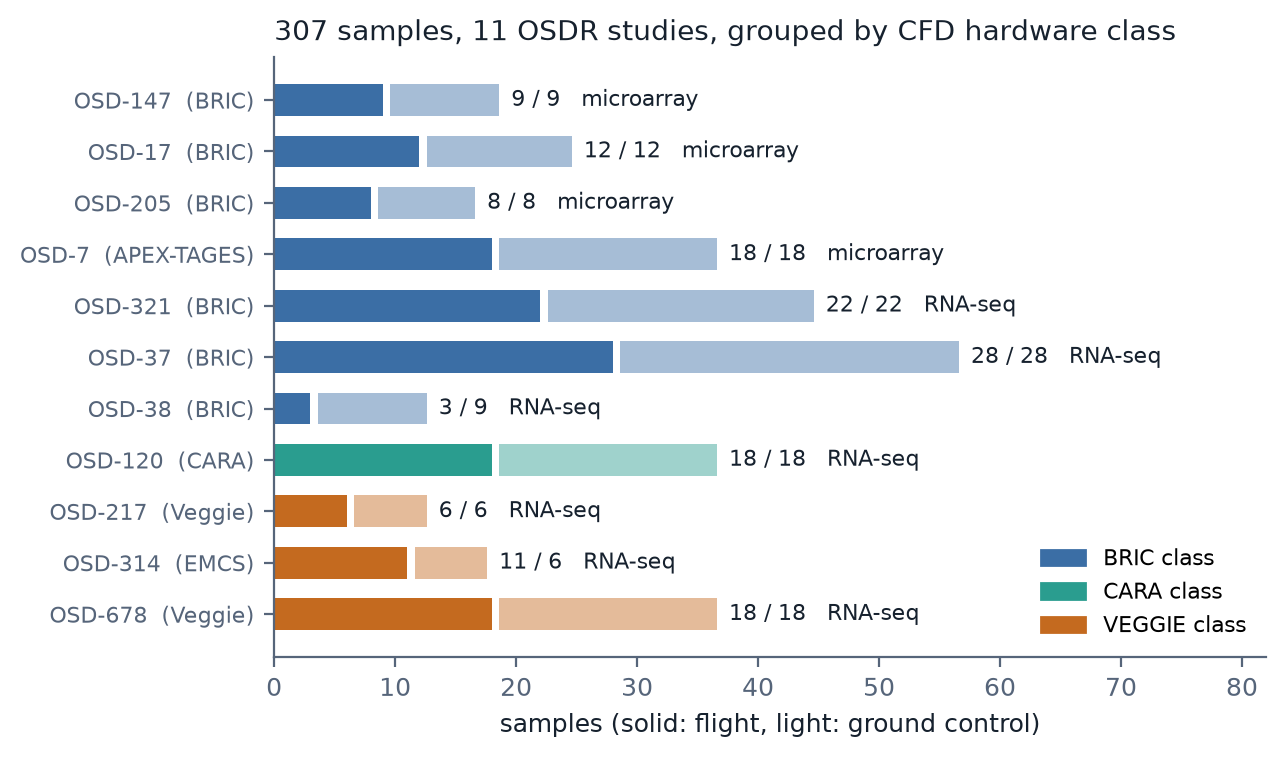
\includegraphics[width=0.9\textwidth]{figures/2026-10/fig1_study_design.png}
\caption{\textbf{Study design.} Flight (solid) and ground-control (light) samples in each of the 11 OSDR studies, coloured by CFD hardware class and labelled by platform. APEX-TAGES (OSD-7) is grouped with BRIC and EMCS (OSD-314) with VEGGIE. Source: \texttt{expression\_metadata\_with\_cfd\_v2.tsv}.}
\label{fig:design}
\end{figure}

\begin{figure}[htbp]
\centering
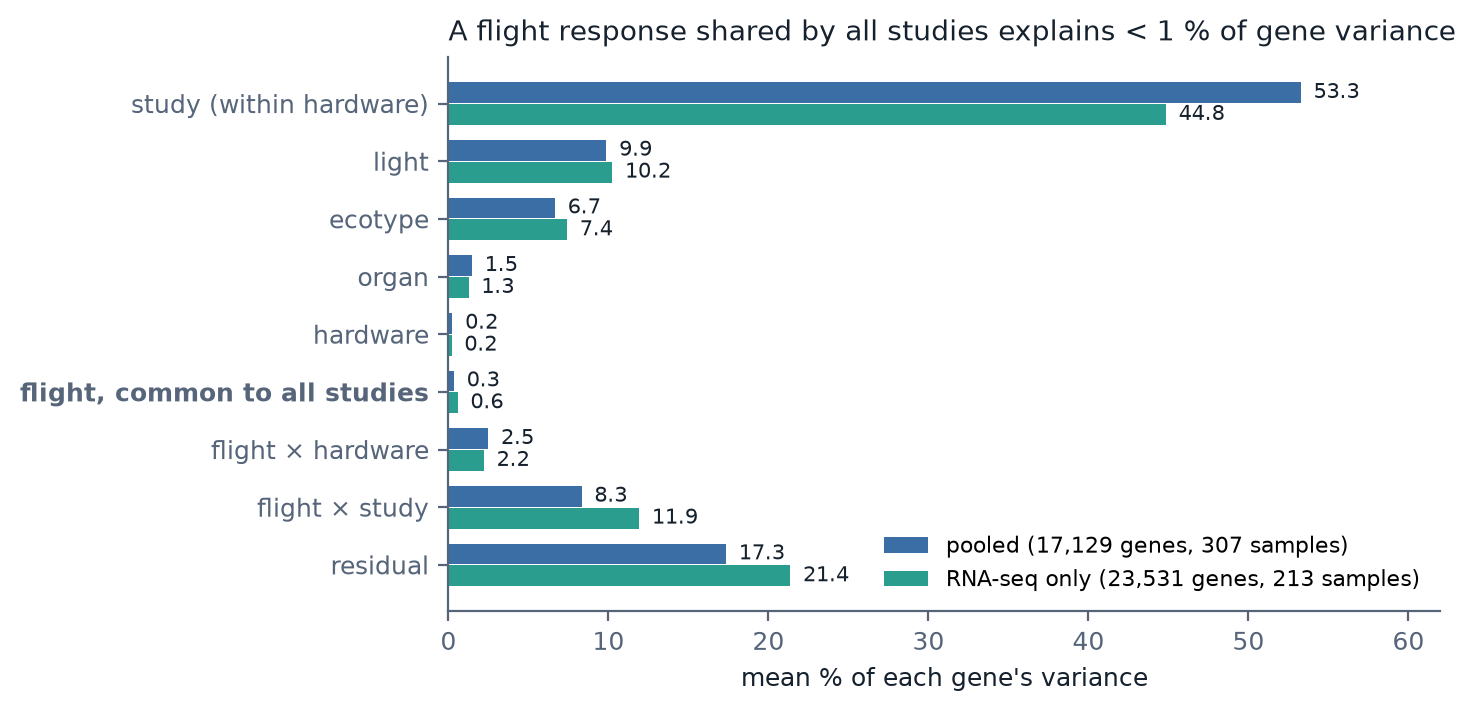
\includegraphics[width=0.9\textwidth]{figures/2026-10/fig2_variance_partition.png}
\caption{\textbf{The flight response is largely study-specific.} Mean percent of each gene's variance explained by each component, for the pooled data (genes measured in all studies) and the RNA-seq studies alone. Every factor is a random effect; hardware is nested in study. Source: REANALYSIS §12.}
\label{fig:vp}
\end{figure}

\begin{figure}[htbp]
\centering
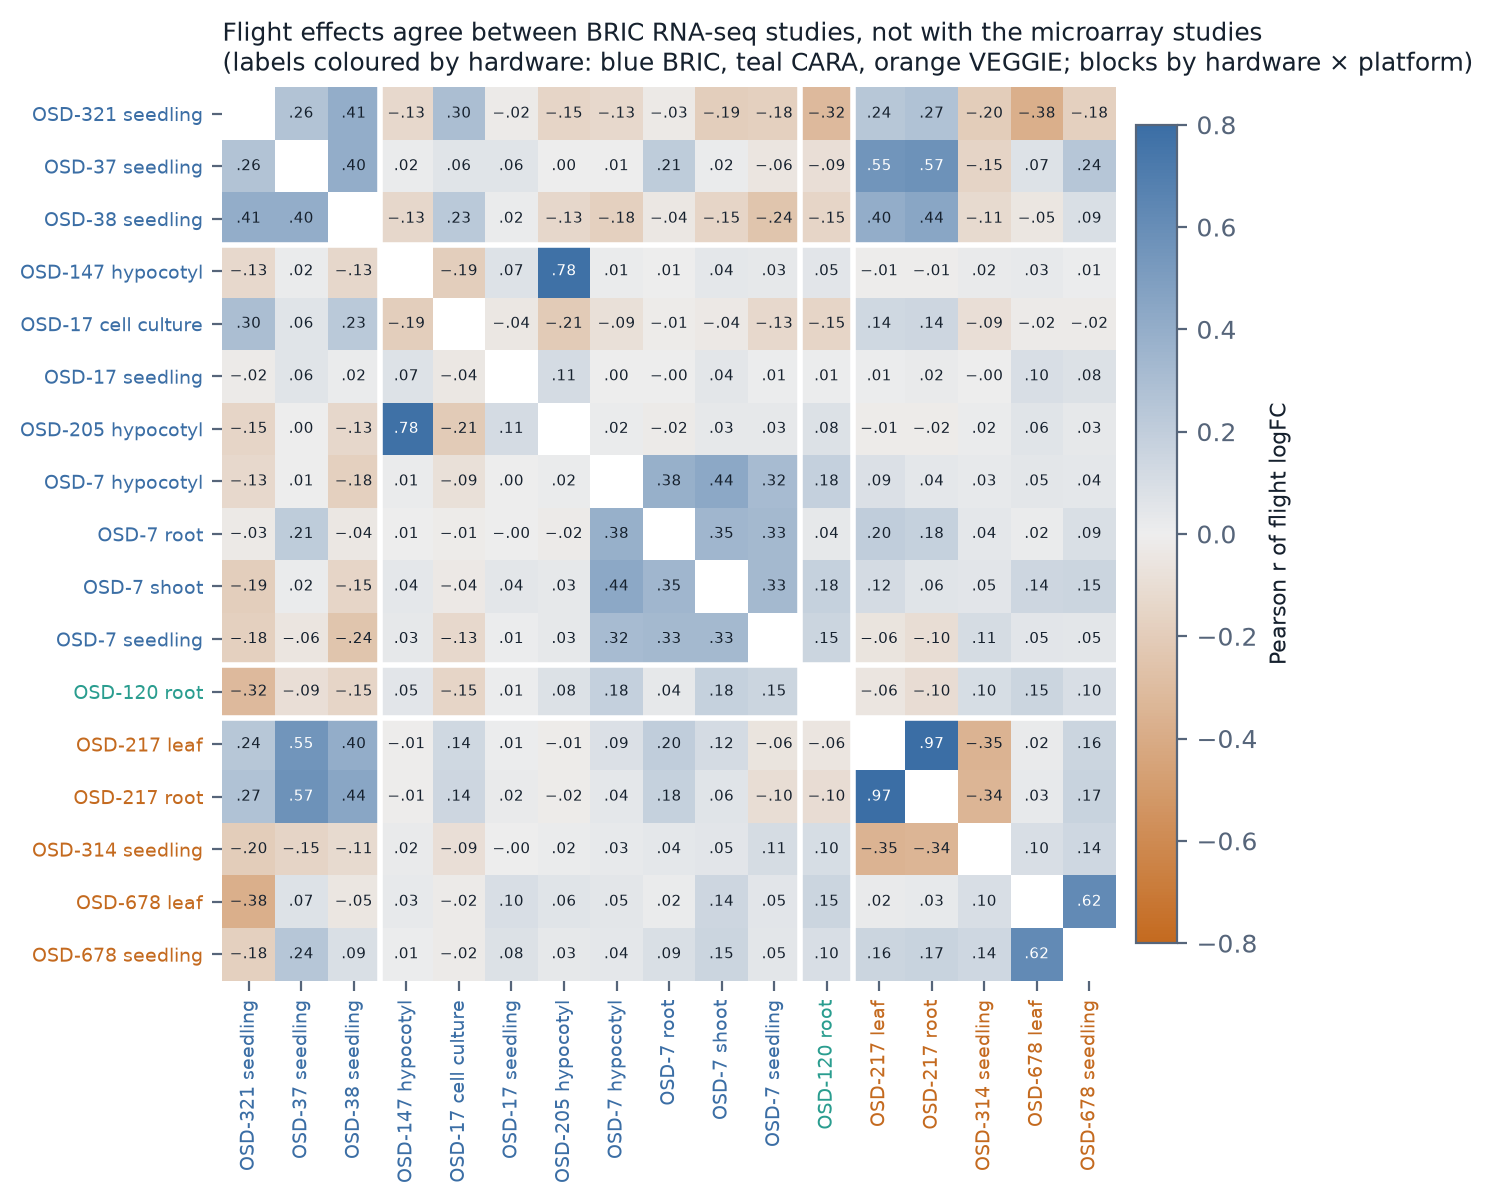
\includegraphics[width=0.9\textwidth]{figures/2026-10/fig3_platform_concordance.png}
\caption{\textbf{Agreement of flight effects between studies.} Pearson correlation of flight $\log_2$ fold changes between study $\times$ organ units, grouped by hardware and platform. BRIC RNA-seq units agree (median $r = 0.40$ between studies); BRIC microarray units agree neither with each other nor with RNA-seq. Source: REANALYSIS §13.}
\label{fig:platform}
\end{figure}

\begin{figure}[htbp]
\centering
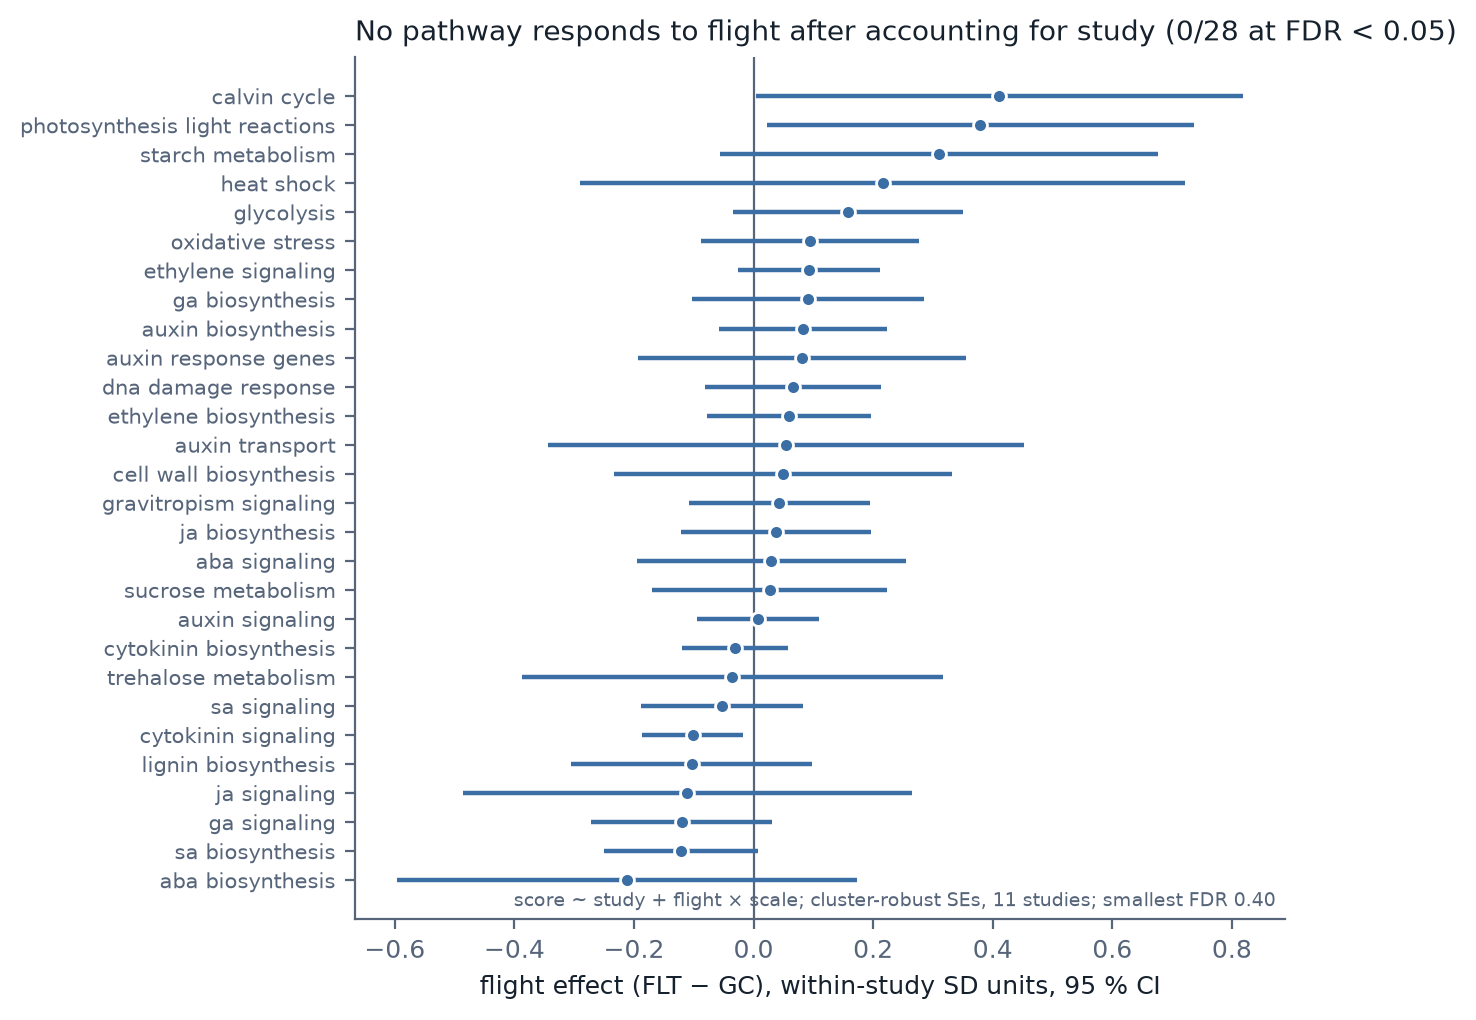
\includegraphics[width=0.85\textwidth]{figures/2026-10/fig4_pathway_flight_effects.png}
\caption{\textbf{No pathway-level flight effect.} Flight effect (flight minus ground) per pathway with 95\% confidence intervals, from a within-study model with cluster-robust errors by study (11 studies), on scores computed within each study without zero-filling. No pathway reaches FDR $< 0.05$. Source: REANALYSIS §10.}
\label{fig:pathways}
\end{figure}

\begin{figure}[htbp]
\centering
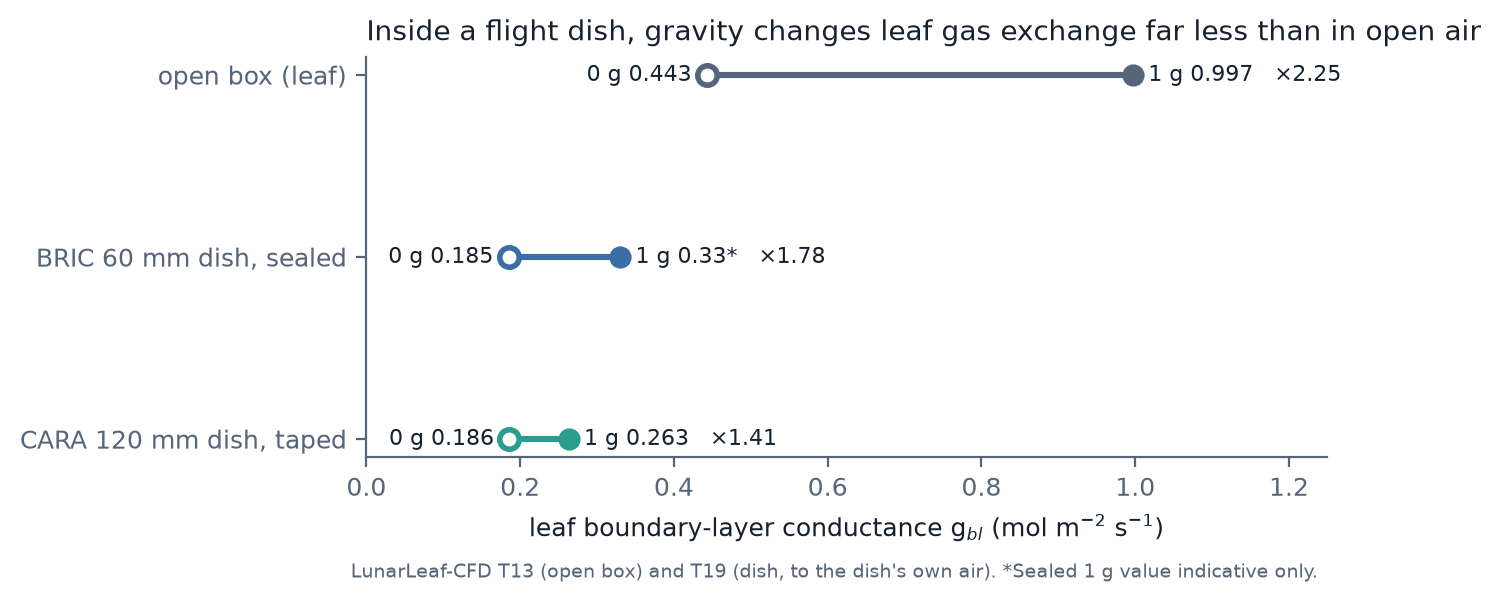
\includegraphics[width=0.9\textwidth]{figures/2026-10/fig5_cfd_dish_penalty.png}
\caption{\textbf{Gravity penalty on leaf gas exchange, open air versus flight dish.} Leaf boundary-layer conductance at 1\,g (filled) and 0\,g (open) in an open box and inside the BRIC and CARA dishes, with the 1\,g/0\,g ratio. The sealed-BRIC 1\,g value is indicative only. Source: LunarLeaf-CFD T13 and T19.}
\label{fig:cfd}
\end{figure}

% ============================================================
% Supplementary tables reference
% ============================================================

\section*{Supplementary Tables}

All in \texttt{tables/reanalysis\_2026-10/}:
\begin{itemize}
    \item Table S1: differential expression for the refit contrasts (\texttt{gene\_level/de\_summary\_v2.tsv} and \texttt{de\_v2\_*.tsv.gz})
    \item Table S2: variance partition per gene and summary (\texttt{followups/variance\_partition\_*})
    \item Table S3: platform concordance, per unit and per pair (\texttt{followups/platform\_concordance\_*})
    \item Table S4: rescored pathway scores and within-study models (\texttt{followups/pathway\_*})
    \item Table S5: meta-regression units and results (\texttt{followups/rescored/})
    \item Table S6: CFD covariates per sample (\texttt{expression\_metadata\_with\_cfd\_v2.tsv})
    \item Table S7: exploratory deconvolution and miRNA inference from the original pipeline (\texttt{tables/deconvolution\_proportions.tsv}, \texttt{tables/mirna\_activity\_inference.tsv})
\end{itemize}

% ============================================================
\bibliographystyle{plainnat}

\begin{thebibliography}{99}

\bibitem[Paul et al., 2017]{paul2017}
Paul, A.-L., Sng, N.J., Zupanska, A.K., Krishnamurthy, A., Schultz, E.R. \& Ferl, R.J. (2017). Genetic dissection of the \textit{Arabidopsis} spaceflight transcriptome: Are some responses dispensable for the physiological adaptation of plants to spaceflight? \textit{PLOS ONE}, 12(6), e0180186. doi:10.1371/journal.pone.0180186

\bibitem[Kitaya et al., 2003]{kitaya2003}
Kitaya, Y., Tsuruyama, J., Shibuya, T., Yoshida, M. \& Kiyota, M. (2003). Effects of air current speed on gas exchange in plant leaves and plant canopies. \textit{Advances in Space Research}, 31(1), 177--182. doi:10.1016/S0273-1177(02)00747-0

\bibitem[Monje et al., 2005]{monje2005}
Monje, O., Stutte, G. \& Chapman, D. (2005). Microgravity does not alter plant stand gas exchange of wheat at moderate light levels and saturating CO\textsubscript{2} concentration. \textit{Planta}, 222(2), 336--345. doi:10.1007/s00425-005-1529-1

\bibitem[Shahan et al., 2022]{shahan2022}
Shahan, R., Hsu, C.-W., Nolan, T.M., Cole, B.J., Taylor, I.W., Greenstreet, L., Zhang, S., Afanassiev, A., Vlot, A.H.C., Schiebinger, G., Benfey, P.N. \& Ohler, U. (2022). A single-cell \textit{Arabidopsis} root atlas reveals developmental trajectories in wild-type and cell identity mutants. \textit{Developmental Cell}, 57(4), 543--560.e9. doi:10.1016/j.devcel.2022.01.008

\bibitem[Lopez et al., 2018]{lopez2018}
Lopez, R. et al. (2018). Deep generative modeling for single-cell transcriptomics. \textit{Nature Methods}, 15, 1053--1058. doi:10.1038/s41592-018-0229-2

\bibitem[Law et al., 2014]{law2014}
Law, C.W. et al. (2014). voom: precision weights unlock linear model analysis tools for RNA-seq read counts. \textit{Genome Biology}, 15, R29. doi:10.1186/gb-2014-15-2-r29

\bibitem[Smyth, 2005]{smyth2005}
Smyth, G.K. (2005). limma: Linear Models for Microarray Data. In: \textit{Bioinformatics and Computational Biology Solutions Using R and Bioconductor}, Springer, pp.~397--420. doi:10.1007/0-387-29362-0\_23

\bibitem[Smyth et al., 2005]{smyth2005b}
Smyth, G.K., Michaud, J. \& Scott, H.S. (2005). Use of within-array replicate spots for assessing differential expression in microarray experiments. \textit{Bioinformatics}, 21(9), 2067--2075. doi:10.1093/bioinformatics/bti270

\bibitem[Robinson \& Oshlack, 2010]{robinson2010}
Robinson, M.D. \& Oshlack, A. (2010). A scaling normalization method for differential expression analysis of RNA-seq data. \textit{Genome Biology}, 11(3), R25. doi:10.1186/gb-2010-11-3-r25

\bibitem[Hoffman \& Schadt, 2016]{hoffman2016}
Hoffman, G.E. \& Schadt, E.E. (2016). variancePartition: interpreting drivers of variation in complex gene expression studies. \textit{BMC Bioinformatics}, 17(1), 483. doi:10.1186/s12859-016-1323-z

\bibitem[Knapp \& Hartung, 2003]{knapp2003}
Knapp, G. \& Hartung, J. (2003). Improved tests for a random effects meta-regression with a single covariate. \textit{Statistics in Medicine}, 22(17), 2693--2710. doi:10.1002/sim.1482

\bibitem[Cameron \& Miller, 2015]{cameron2015}
Cameron, A.C. \& Miller, D.L. (2015). A practitioner's guide to cluster-robust inference. \textit{Journal of Human Resources}, 50(2), 317--372. doi:10.3368/jhr.50.2.317

\bibitem[Benjamini \& Hochberg, 1995]{benjamini1995}
Benjamini, Y. \& Hochberg, Y. (1995). Controlling the false discovery rate: a practical and powerful approach to multiple testing. \textit{Journal of the Royal Statistical Society Series B}, 57(1), 289--300. doi:10.1111/j.2517-6161.1995.tb02031.x

\end{thebibliography}

\end{document}
